This section details the characterization of the SiPM S13360-1375 model, which was the first choose for the TRITIUM monitor photosensors. It has to be taken into account that this characterization is incomplete since some important SiPM parameters for the TRITIUM monitor, which are its PDE, its dark count rate and its crosstalk probability, was not experimentally measured. 

A complete characterization is already underway for the S13360-6075 model, the latest proposal for the TRITIUM detector, where all interesting parameters, which are explained in section \ref{subsubsec:SiPM}, will be experimentaly determined using a different experimental setup, shown in appendix \ref{App:ElectronicReadoutSiPM}.

The SiPM characterization is carried out inside of a climatic chamber, model CCM 81 from DYCOMETAL \cite{ClimaticChamberIFIMED}. This climatic chamber allow to control the temperature and humidity with a precisión of $0.1\celsius$ and $0.1\%$ respectively. In addition, this is metallic, acting as a Faraday cage, and a special black blanket \cite{BlackBlancket} was used to prevent external photons from reaching the SiPM.

First of all the the quenching resistance and the breakdown voltage of the SiPM were experimentally obtained. Both parameters can be calculated from the measurement of the current-voltage curves of the SiPM, bias voltage applied in forward and reverse direction respectively. This measurement should be done without the amplification of the electronic board to achieve a better precision and without illuminating the SiPM. Therefore, the output current of the SiPM was directly measured using the Keithley 6487 Picoammeter/Voltage Source \cite{DataSheetKeithley6487} and the LabView program was used to automate the taking of measurements. The results of both measurements are plotted as a function of the bias voltage applied in Figure \ref{fig:IVcurveSiPM}.

\begin{figure}
\centering
    \begin{subfigure}[b]{0.9\textwidth}
    \centering
    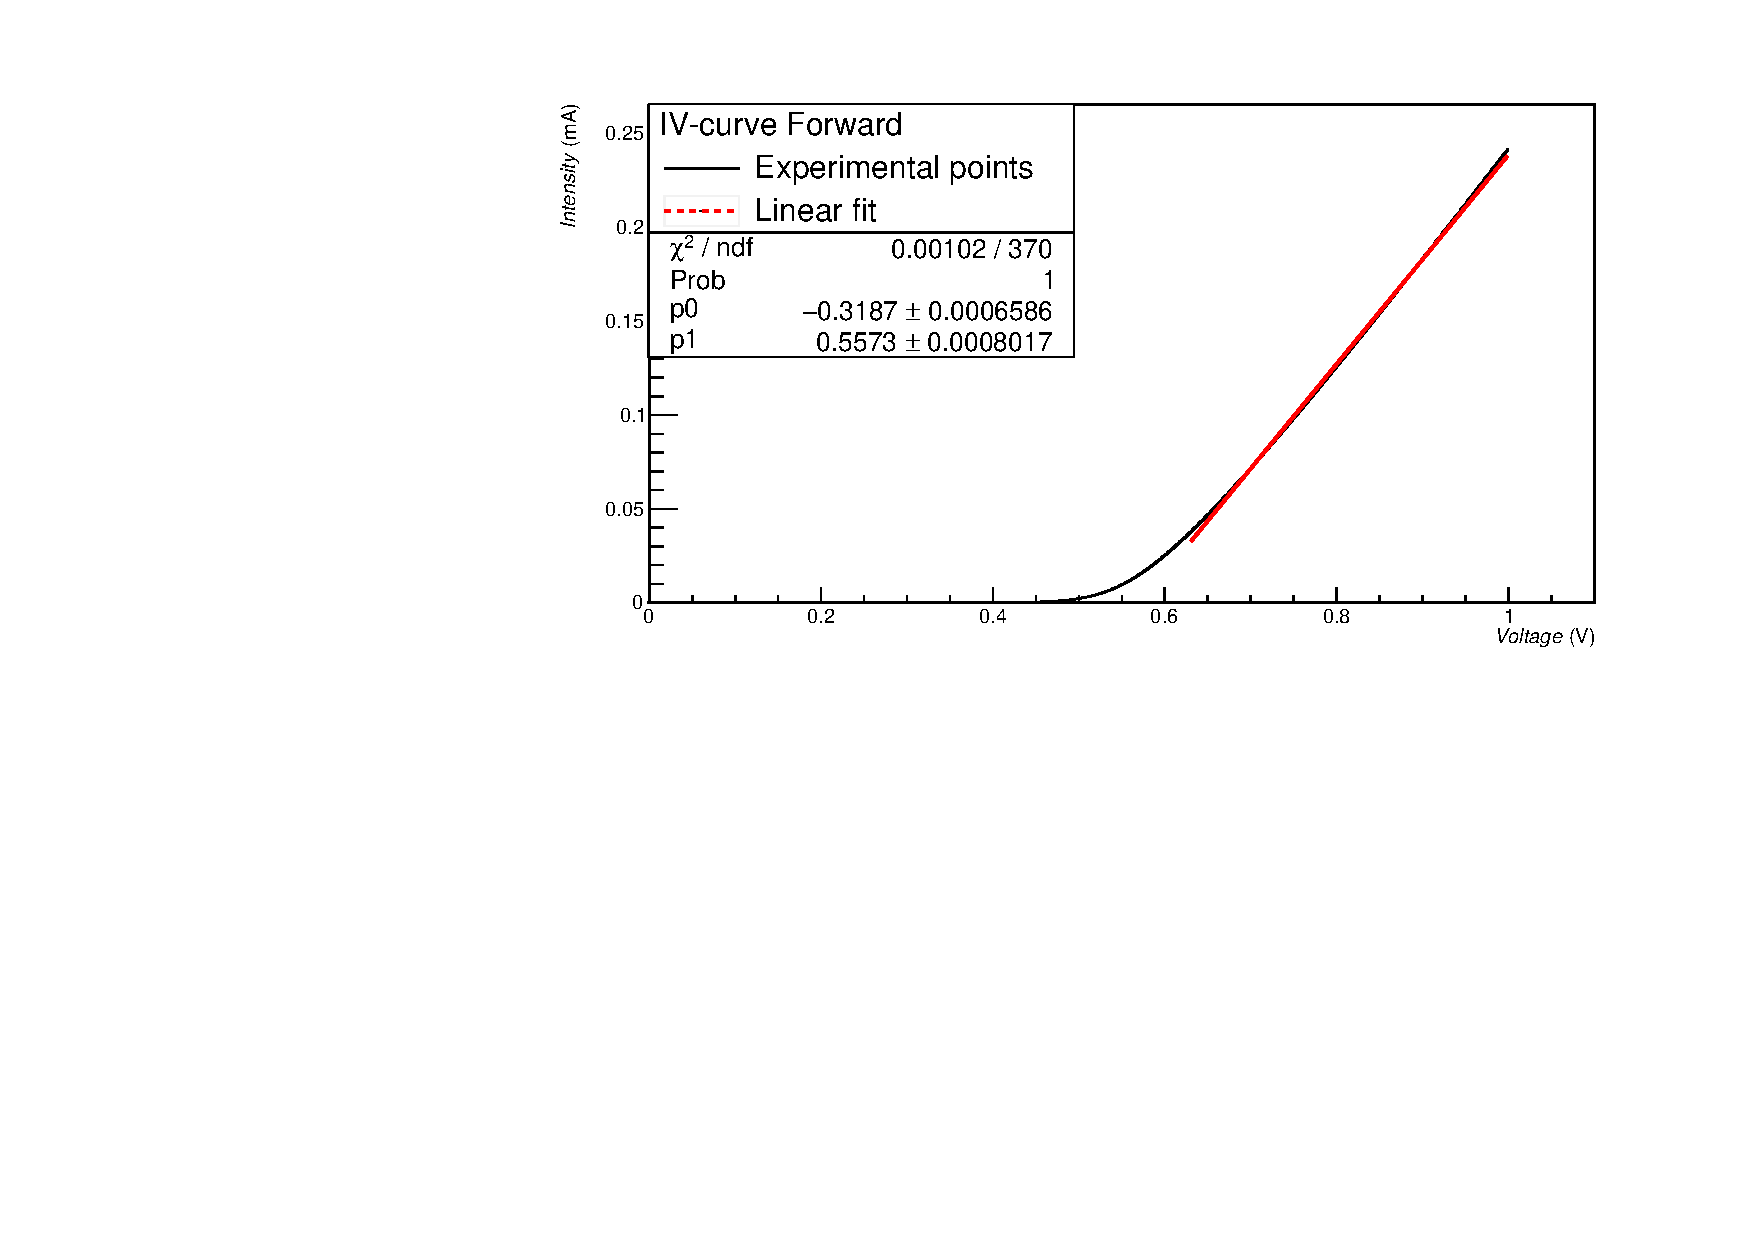
\includegraphics[width=\textwidth]{4ResearchAndDevelopments/42SiPM/IVCurveSiPMForward.pdf}  
    \caption{\label{subfig:IVcurveForward}}
    \end{subfigure}
    \hfill
    \begin{subfigure}[b]{0.9\textwidth}
    \centering
    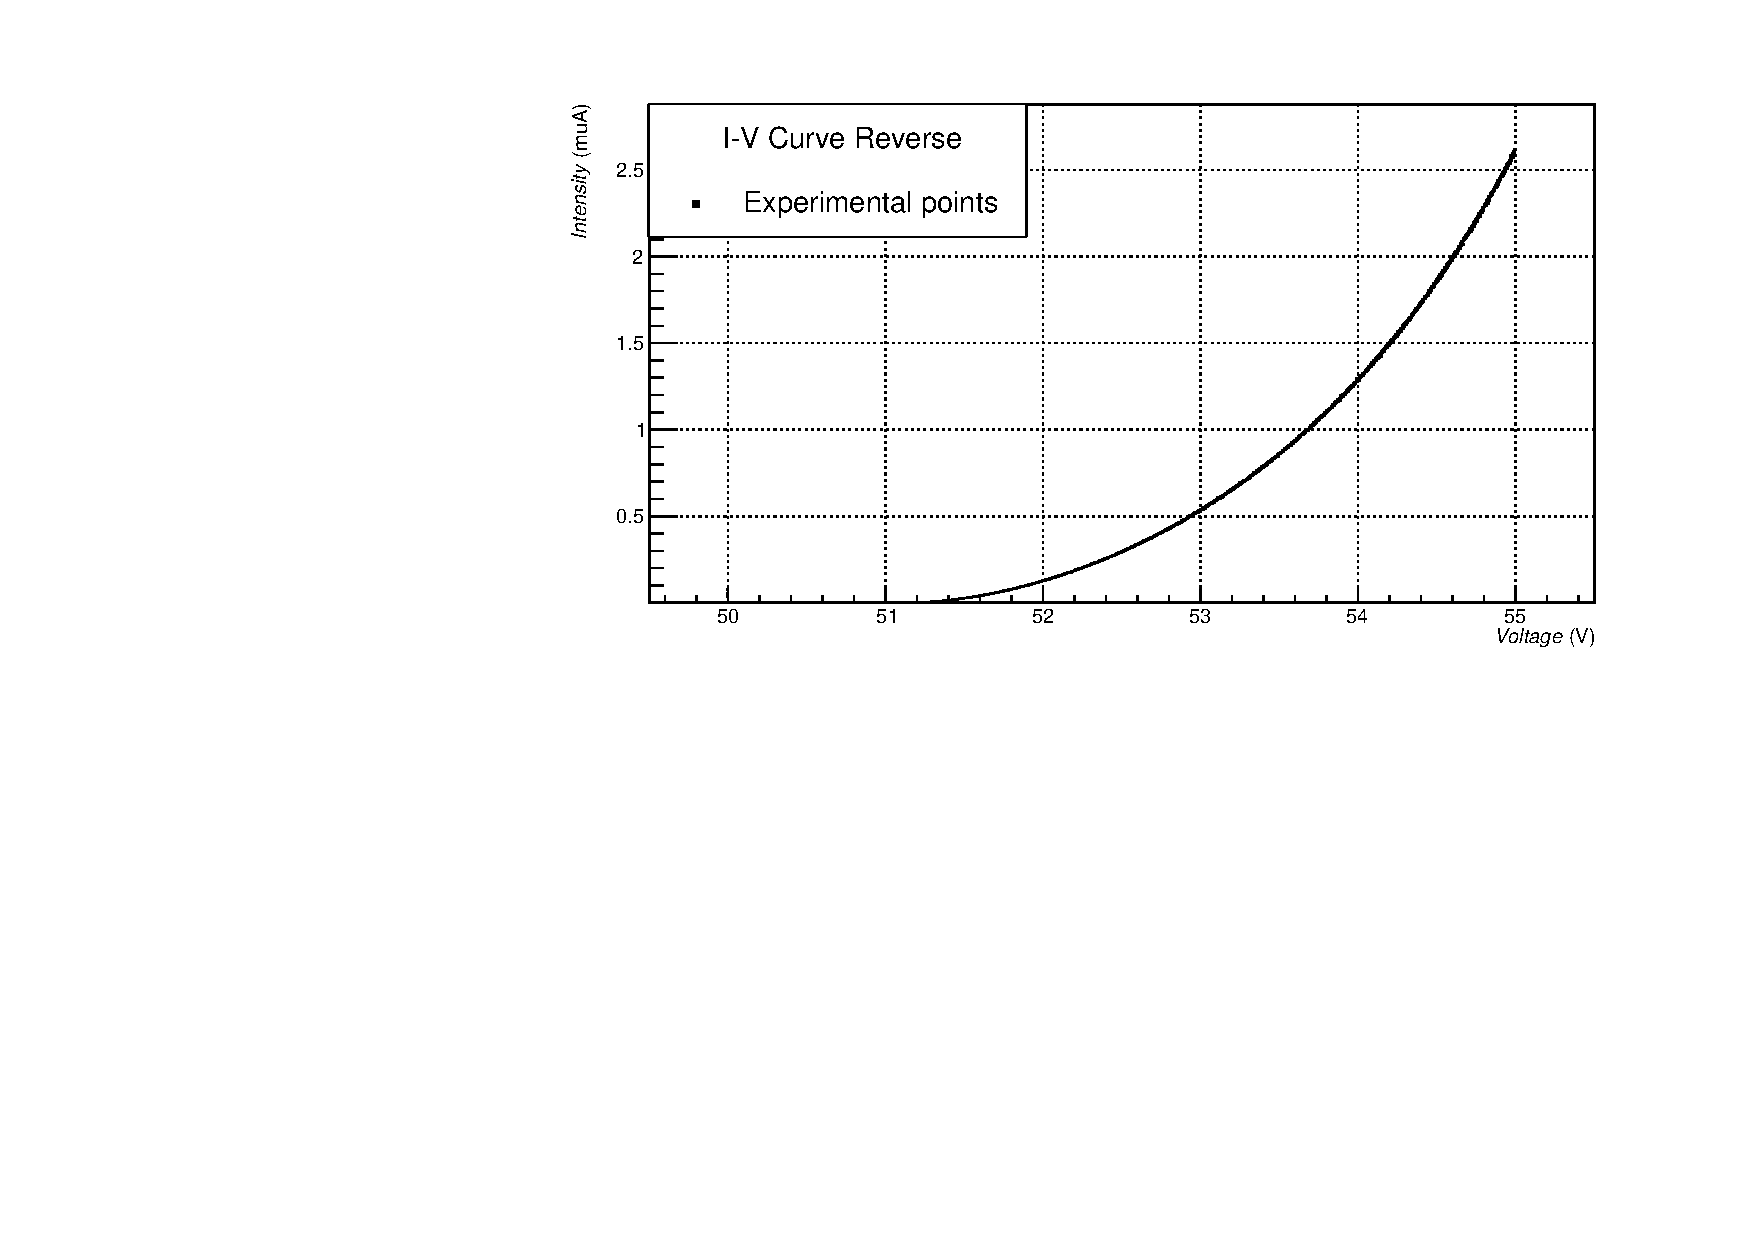
\includegraphics[width=\textwidth]{4ResearchAndDevelopments/42SiPM/IVCurveSiPMReverse.pdf}  
    \caption{\label{subfig:IVcurveReverse}}
    \end{subfigure}
 \caption{I-V curves measured for the SiPM S13360-1375 model with the Bias voltage applied in a) forward direction b) reverse direction. This experience was carried out at $T=25\celsius$ and humidity of $H=45\%$}
 \label{fig:IVcurveSiPM}
\end{figure}

As can be seen when the bias voltage is applied in forward direction, Figure \ref{subfig:IVcurveForward}, the output current of the SiPM doesn't flow until the potencial difference existing between the n and p layers are reached, which is approximately $V_0=0.7~\volt$ for silicon photosensors, quite similar to the value experimentally obtained, $V_0= 0.5~\volt$. When the current start to flow, the intensity is linear with the applied voltage following the equation:
\begin{equation}
I=\frac{1}{R_{eq}}V;  \qquad \frac{1}{R_{eq}} = \sum_{i=1}^{N}\frac{1}{R_{qi}}= \frac{N}{R_{q}}
\label{QuenchingResistance}
\end{equation}
Where $R_{eq}$ is the equivalent resistance of all quenching resistance of the SiPM, $R_{q}$, which are in parallel. Therefore, a value of $R_{q}= 511.39 \pm 0.74~\kilo\ohm$ is experimentaly obtained, which is in agreement with the typical values used by Hamamatsu.

Regardness to the experience where a reverse bias voltage was applied, the output current of SiPM start to flow when the breakdown voltage is reached, which can be calculated from the maximum of the function 
\begin{equation}
f=\frac{1}{I}\frac{dI}{dV}
\label{BreakDownVoltageFunction}
\end{equation}

The value obtained is $V_{BD}=51.02~\volt$, quite in agreement with the value providad by Hamamatsu, Table \ref{tab:PropertiesOfSiPM1375}.

Now, to experimentally measure the SiPM gain, $G_{SiPM}$, the electronic board shown in section \ref{subsubsec:SiPMsElectronicalSystem} was used, with which an amplification factor of $F_{amp}=170$ is applied. An incoherent light source, LED435-03 from Toithner LaserTechnik Gmbh \cite{LEDRLT}, the characteristics of which is described in section \ref{subsec:CharacterizationFibers}, is used to illuminate the SiPM with a low enough density of $\lambda= 435~\nm$ photons.

When the incoherent light source is used, the SiPM output signal shows various well-defined heights, shown in Figure \ref{fig:OutputPulses_SPSspectrum} above, according to several fired pixels simultaneously. Then, the single photon spectrum, SPS, shown in Figure \ref{fig:OutputPulses_SPSspectrum} below, was obtained. This is done by integring and hitogramming the SiPM output pulses using time windows wide enough to ensure that the charge of the pulse is fully contained. The time windows used in this experience was $t_w= 500~\nano\second$. A trigger signal is used, green signal in Figure \ref{fig:OutputPulses_SPSspectrum}, which indicates when de light source is iluminating the SiPM.

\begin{figure}[hbtp]
\centering
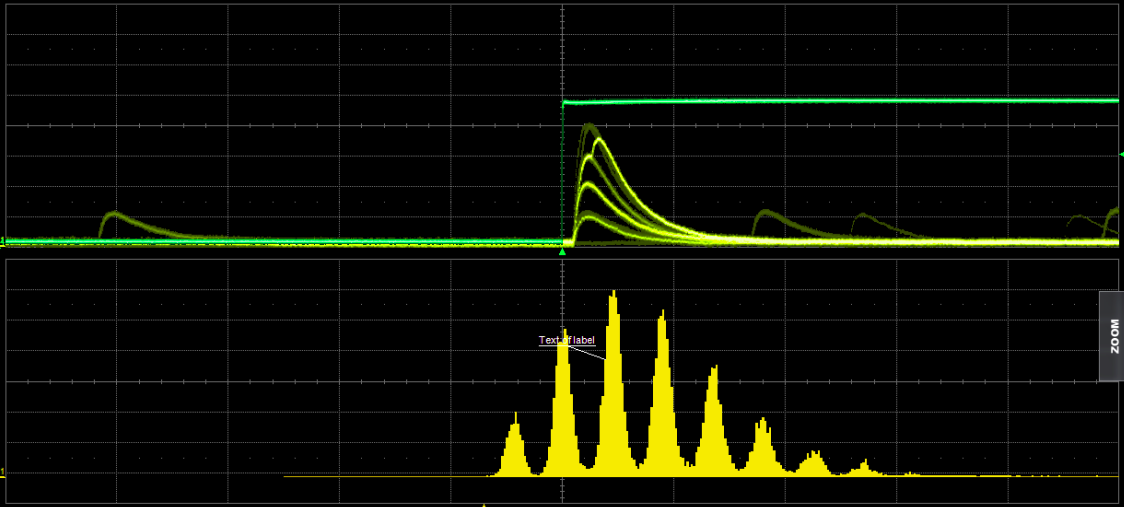
\includegraphics[scale=0.3]{4ResearchAndDevelopments/42SiPM/SiPMPulses_SPS_Spectrum.png}
\caption{Above: Trigger signal (green) and SiPM output pulses (yellow) diplayed on the oscilloscope, model WwaveRunner 625Zi from TELEDYNE LECROY \cite{OscilloscopeIFIMED}, in which the persistence function is used. Bottom: SPS spectrum obtained by integring and histograming the SiPM output pulses. This measurement was done at $25\celsius$, $V_{bias}=53.98$ and humidity of $60\%$. \label{fig:OutputPulses_SPSspectrum}}
\end{figure}

As can be seen, several well-separated peaks are obtained in the SPS spectrum. Each peak exhibits the charge produced by a different number of fired pixels (detected photons). It has to be taken into account that the left-most peak in the spectrum is the so-called pedestal, which is the charge when no pixels are fired. This peak is caused by the electronic noise of the system and this should not be included in the analysis explained below. The second peak corresponds to one fired pixel and so on.

The SiPM Gain, $G_{SiPM}$, can be extrapolated from the SPS spectrum using the equation:
\begin{equation}
G=\frac{\overline{\Delta Q (V \cdot{} s)}}{F_{amp}(V/A) \times q_{e^-}(C)}
\label{SiPMGain}
\end{equation}
where $q_{e^-}$ is the electron charge and $\overline{\Delta Q (Vs)}$ is the average of the distastance between the peaks of the SPS spectrum, which is the charge due to one fired pixel. 

To measure the value of $\overline{\Delta Q}$ a script was written using the ROOT program \cite{ROOTWebPage} developed by CERN and the TSpectrum library was included for data analysis. 

First, this script find and extract the bakcground, which, in some cases like high temperatures or high bias voltages, can lead to erroneous analysis of the data. Then, this macro find all peaks in the SPS spectrum and fits each one to a Gaussian funtion, shown in Figure \ref{subfig:GaussianFitSiPMs}. The value and error of the charge produced by multiple fired pixels are obtained from the centroid and the sigma of the different fitted Gaussian functions. Finally, the obtained charges are adjusted to a succesive number of fired pixels, Figure \ref{subfig:LinearFitSiPMGain}, where errors are include but they are too small to be visible.

\begin{figure}
\centering
    \begin{subfigure}[b]{0.47\textwidth}
    \centering
    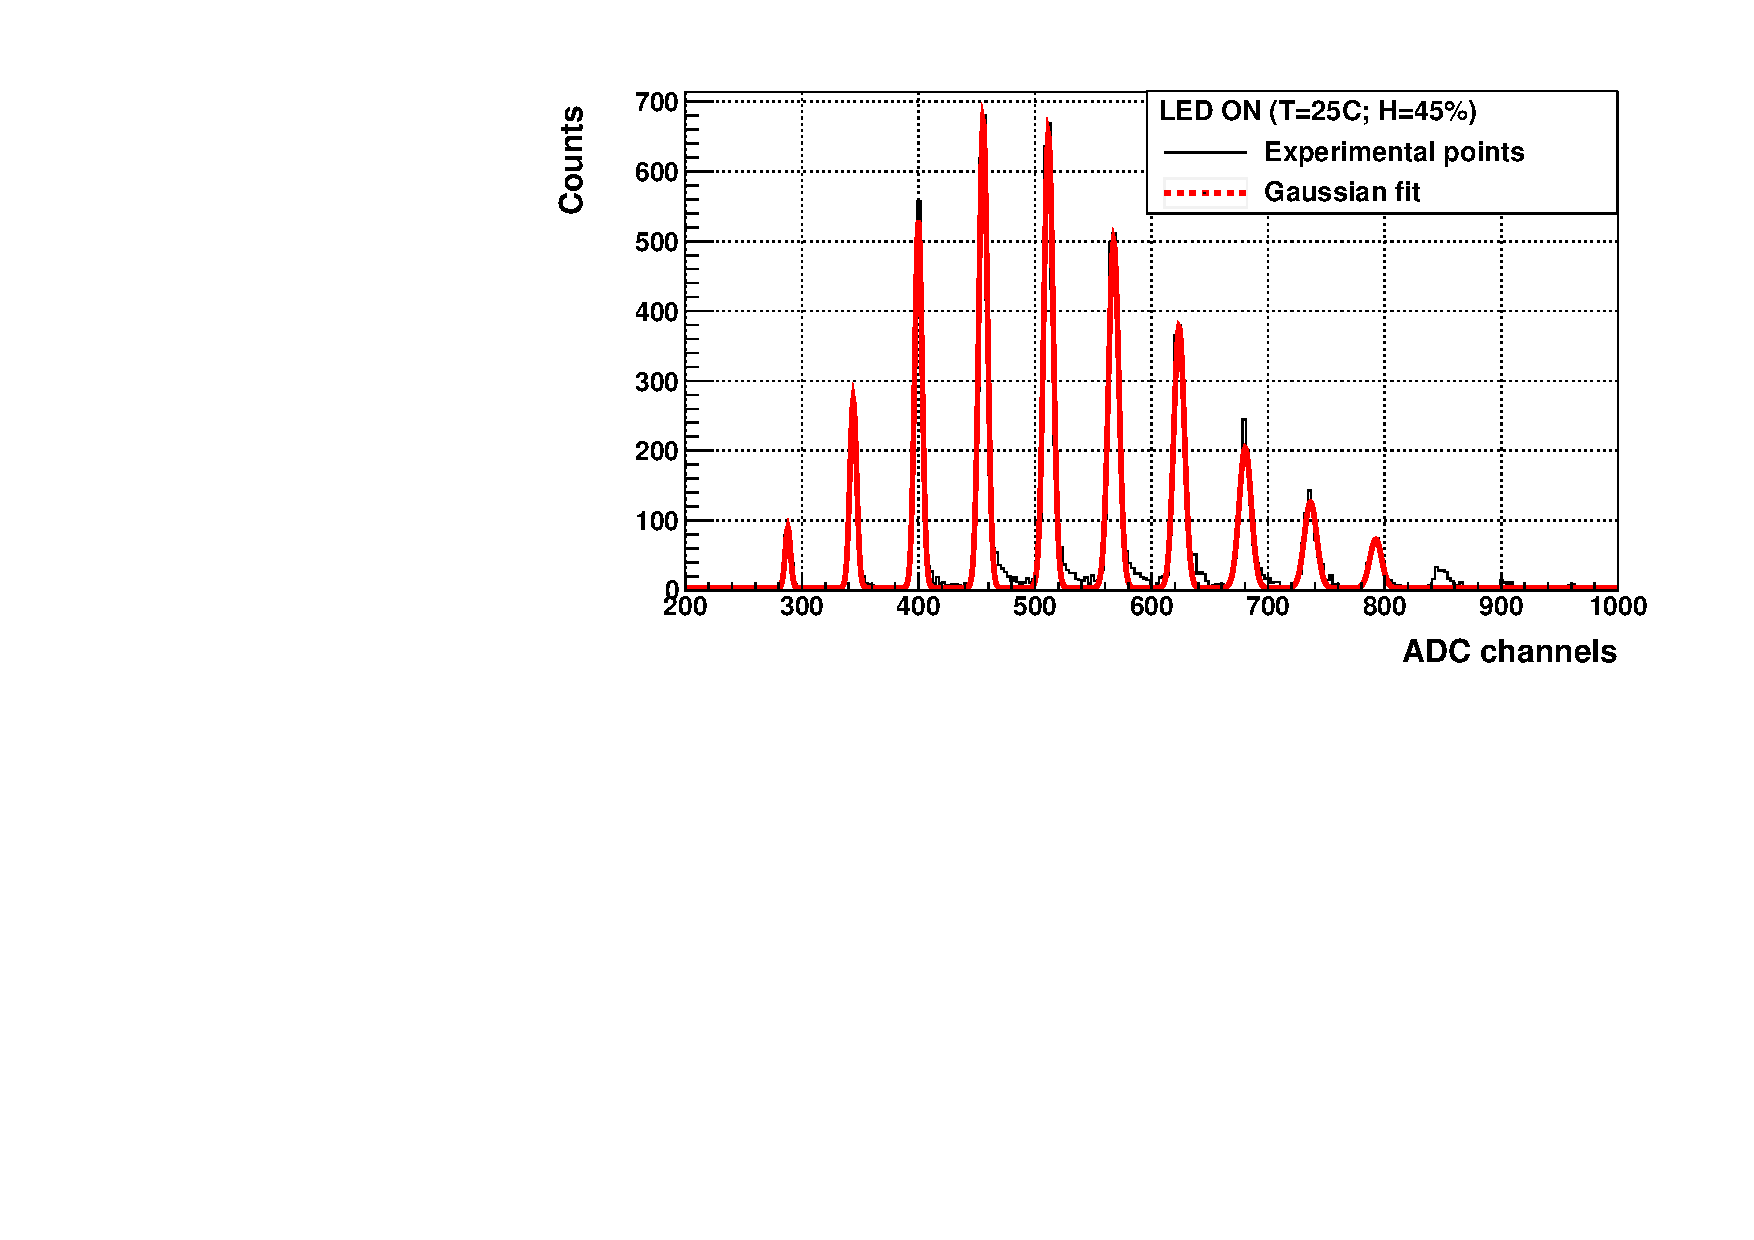
\includegraphics[width=\textwidth]{4ResearchAndDevelopments/42SiPM/GaussianFitSPSSpectrum.pdf}  
    \caption{\label{subfig:GaussianFitSiPMs}}
    \end{subfigure}
    \hfill
    \begin{subfigure}[b]{0.47\textwidth}
    \centering
    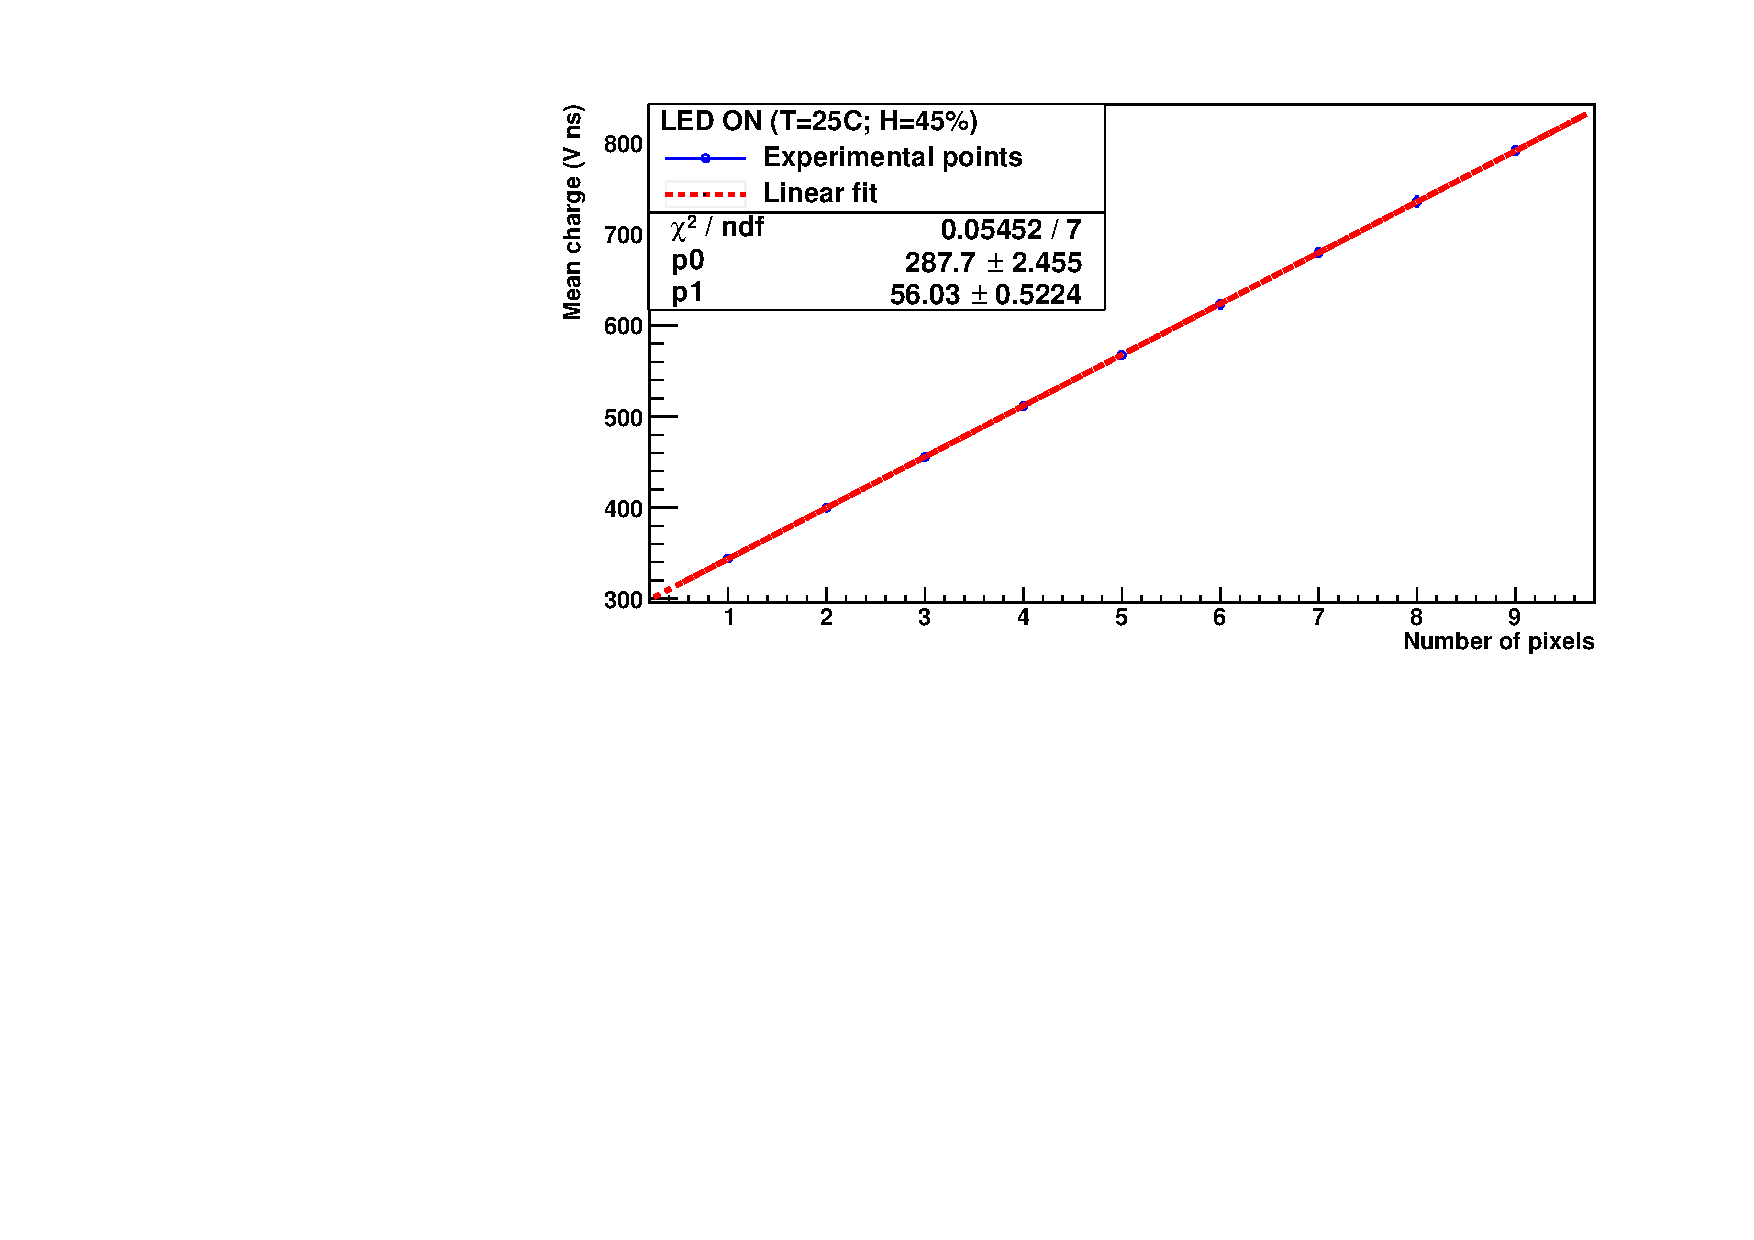
\includegraphics[width=\textwidth]{4ResearchAndDevelopments/42SiPM/LinearFit_Gain_NPixels.pdf}  
    \caption{\label{subfig:LinearFitSiPMGain}}
    \end{subfigure}
 \caption{ROOT analysis performed to obtian the SiPM gain. a) Fit of the SPS spectrum to various Gaussian functions. b) Charge of succesive number of pixels as a function of the number of pixels fired. This experience was carried out at $T=25\celsius$, $V_{bias}=53.98~\volt$ and humidity of $H=45\%$}
 \label{fig:ROOTAnalysisSiPMGain}
\end{figure}

As can bee seen in Figure \ref{subfig:GaussianFitSiPMs}, a very good fit is achieved by the ROOT script with a $\chi^2$ test of $\frac{\chi^2}{ndf}=\frac{1276}{223}$. Up to 10 simultaneously fired pixels has been obtained with a relative uncertainty of the charge measurement of less than $2\%$. An excellent fit is also obtained in Figure \ref{subfig:LinearFitSiPMGain} ($\frac{\chi^2}{ndf}=\frac{0.05452}{7}$), the slope of which correspond to the $\overline{\Delta Q}$.

Therefore, for the case measured at the temperature of $25\celsius$, humidity of $H=45\%$ and overvoltage $V_{OV}=3~\volt$, the value obtained for the SiPM gain is $G_{SiPM}=4,11\cdot{} 10^{6}$, very close to the value provided by Hamamatsu, Table \ref{tab:PropertiesOfSiPM1375}.

Finally, a stabilization method for the SiPM gain is tested. This is necessary for the TRITIUM project since the temperature of the final emplacement of the tritium detector cannot be controlled with enough sensitivity to ensure that it does not affect the SiPM gain and, therefore, the tritium measurement. 

This method consists of compensating for variations in the SiPM gain caused by variations in temperature using controlled variations in the bias voltage. For this task, first, the dependence of the SiPM gain with the temperature and bias voltage is experimentally obtained. To do so, on the one hand, the SiPM gain was measured at several temperatures in the range of $[15-41]\celsius$ with steps of $2\celsius$, which is expected to be the temperature range in the final emplacement. The bias voltage used was $V_{bias} = V_{BD}+3$. On the other hand, the SiPM gain was measured at several bias voltage in the range of $[V_{BD}+1-V_{BD}+5]~\volt$ with steps of $0.2~\volt$, wide enough range to obtain the relationship. The temperature used was $T=25\celsius$. Both measurements are shown in Figure \ref{fig:SiPMGainDependance} in which a linear fit was applied. 

\begin{figure}
\centering
    \begin{subfigure}[b]{0.47\textwidth}
    \centering
    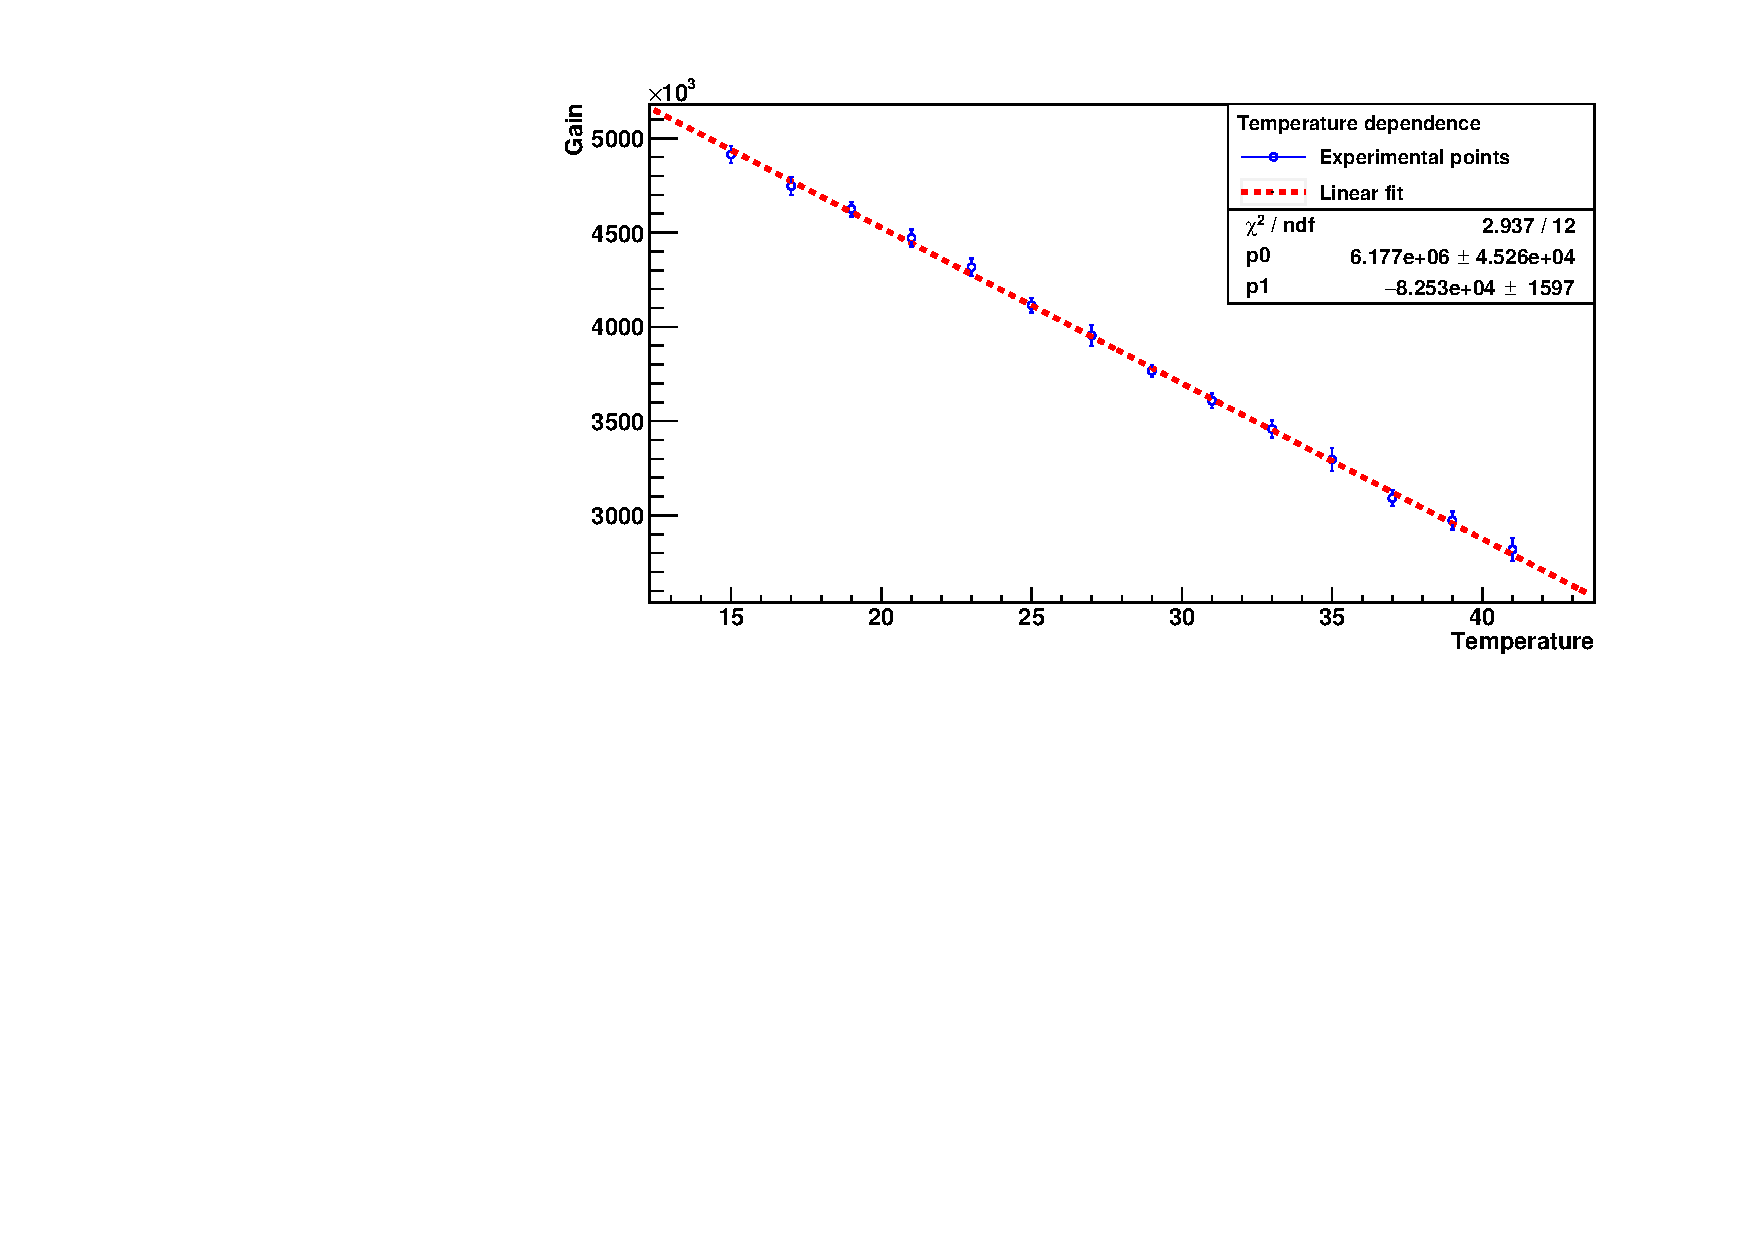
\includegraphics[width=\textwidth]{4ResearchAndDevelopments/42SiPM/SiPMGain_vs_Temperature.pdf}  
    \caption{\label{subfig:SiPMGainvsTemperature}}
    \end{subfigure}
    \hfill
    \begin{subfigure}[b]{0.47\textwidth}
    \centering
    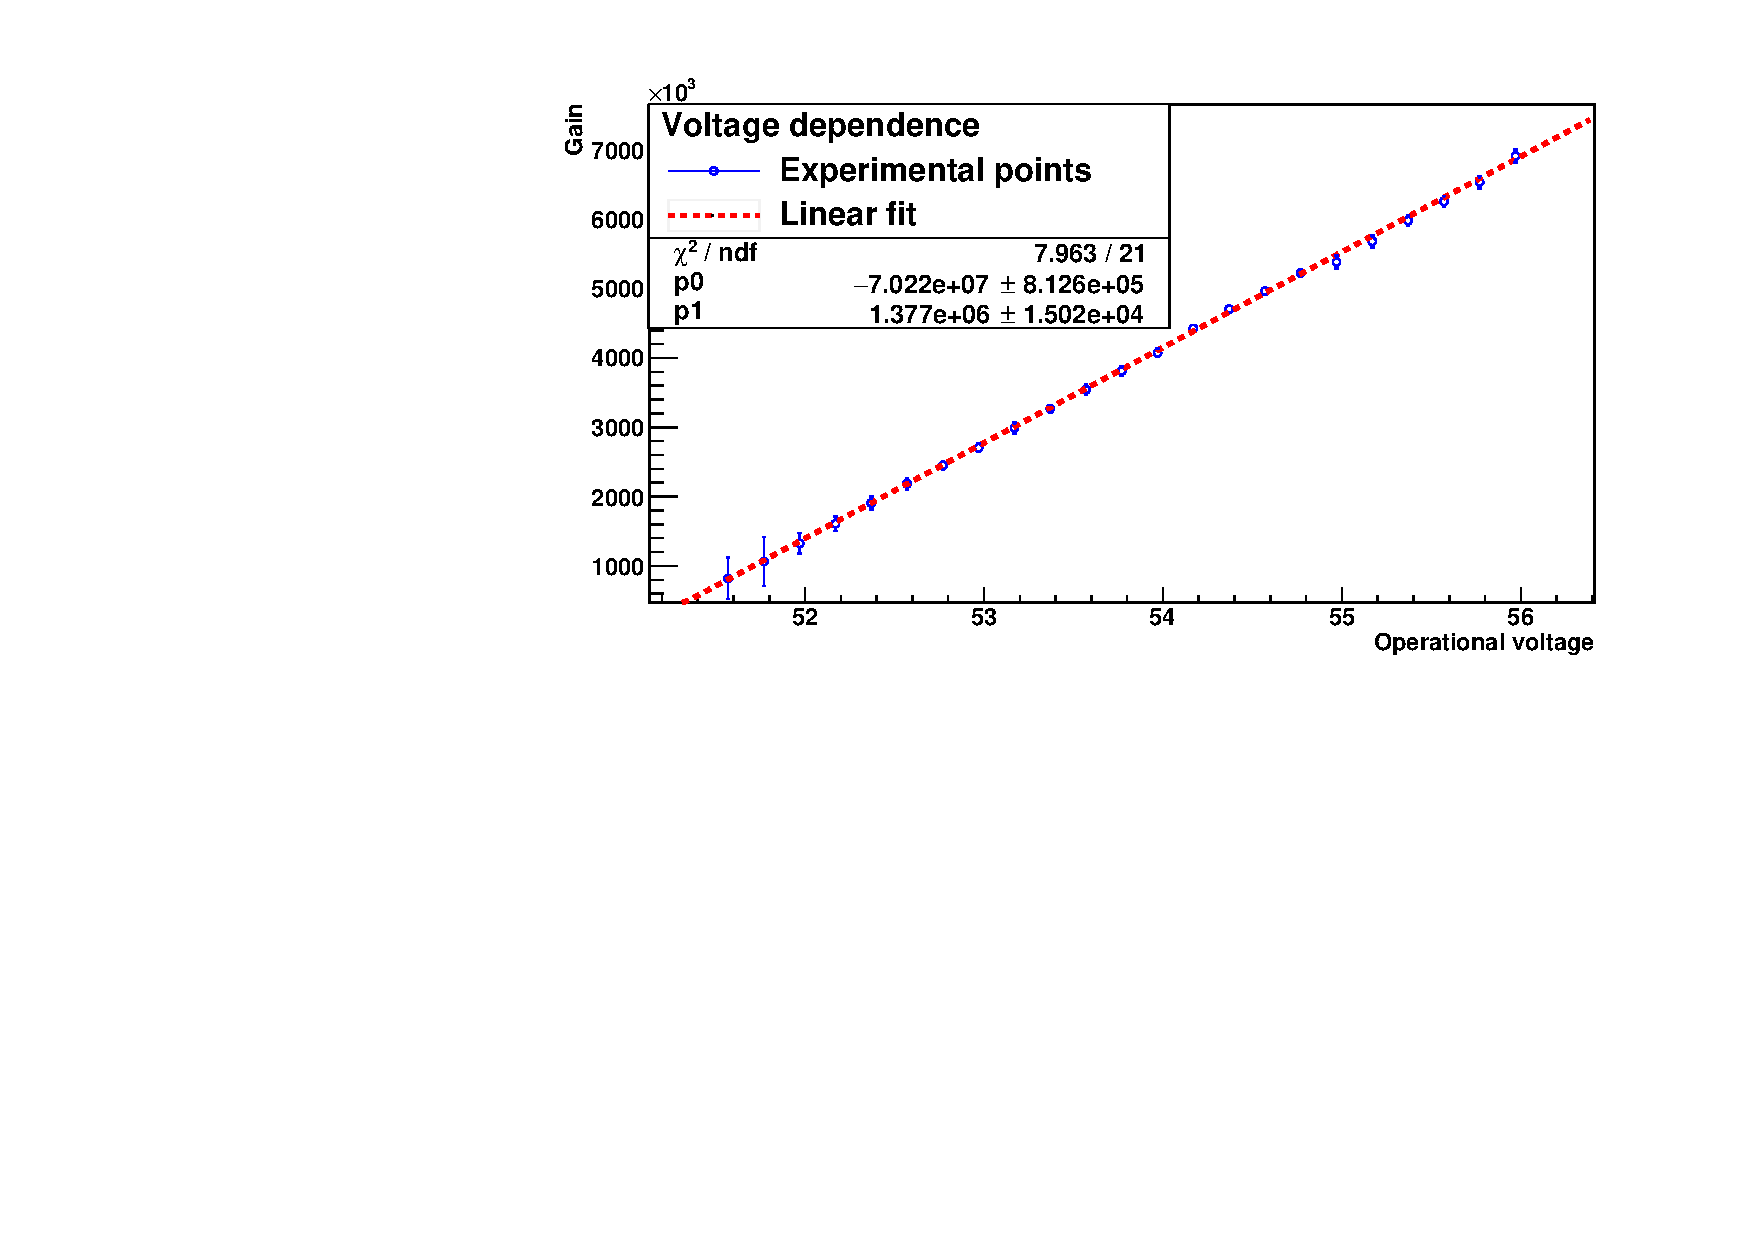
\includegraphics[width=\textwidth]{4ResearchAndDevelopments/42SiPM/SiPMGain_vs_Bias_Voltage.pdf}  
    \caption{\label{subfig:SiPMGainvsBiasVoltage}}
    \end{subfigure}
 \caption{Dependence of the SiPM gain with the a) Temperature b) Bias votlage.}
 \label{fig:SiPMGainDependance}
\end{figure}

As can be seen, a very good linear trend is obtained for both cases, exhibit in the equation \ref{SiPMGainVSTempV}, with values obtained for the $\chi^2/ndf$ variable of $2.937/12$ and $7.963/21$ respectively. The linear fit obtained for both tests are:
\begin{equation*}
\begin{split}
G_{SiPM}=a \cdot{} T + b;& \qquad G_{SiPM}=c \cdot{} V_{bias} + d\\
a=\left( -82.53 \pm 1.59 \right) \cdot{} 10^{3};& \qquad c=\left( 137.72 \pm 1.50 \right) \cdot{} 10^{4}\\
b=\left( 617.65 \pm 4.53 \right) \cdot{} 10^{4};& \qquad d=\left( -762.16 \pm 8.13 \right) \cdot{} 10^{5} \\
\label{SiPMGainVSTempV}
\end{split}
\end{equation*} 

In addition, the breakdown voltage, $V_{BD}$ and the terminal capacitance $C_t$ can be obtained from the linear fit of the SiPM gain as a function of the bias voltage, $V_{bias}$. Both parameters can be calculed through the definition of the SiPM gain and taking into account that, in a parallel plate capacitor, the charge produced in a pixel is directly proportional to the terminal capacitance of the pixel and the difference voltage in the SiPM:
\begin{equation}
G_{SiPM}=\frac{Q_{pixel}}{e^-} = C_d \frac{V_{bias}-V_{BD}}{e^-} = c \cdot{} V_{bias}+d
\label{SiPMGain_Capacitance}
\end{equation}
where $C_d$ is the capacitance of one pixel.

Therefore, using the linear fit obtained in Figure \ref{subfig:SiPMGainvsBiasVoltage}, a value of $V_{BD}=50.98 \pm 0.59~\volt$ and $C_d{}= 220.63 \pm 2.41~\text{f}\farad$ are obtained. The terminal capacitance of the SiPM can be calculated considering all pixels in parallel, $C_{t}=N_{p}\times C_{d}=62.88 \pm 0.69~\pico\farad$. Both parameters, the breakdown voltage and the terminal capacitance, are agree with the values provided by Hamamatsu, Table \ref{tab:PropertiesOfSiPM1375}. 

Finally, the value of the bias voltage to be applied to compensate for the variation in the SiPM gain due to a variation in the temperature can be obtained from both linear trends of Figure \ref{fig:SiPMGainDependance}, applying variations to them:
\begin{equation*}
\begin{split}
G_{SiPM}=a \cdot{} T + b  &\longrightarrow \partial G_{SiPM}= a \partial T\\
G_{SiPM}=c \cdot{} V_{bias} + d &\longrightarrow \partial G_{SiPM}= a \partial V_{bias}
\label{Gain_compensationVariations}
\end{split}
\end{equation*} 

Therefore, the total variation of the SiPM gain, which is produced by the variation of both parameters, must be equal to zero:
\begin{equation*}
\begin{split}
\partial G_{SiPM, tot}= \partial G_{SiPM}(T) &+ \partial G_{SiPM}(V_{bias}) = 0\\ 
\partial G_{SiPM}(V_{bias}) = -\partial G_{SiPM}(T) &\longrightarrow c \partial V_{bias} = - a \partial T\\ 
\partial V_{bias}  = - \frac{a}{c}&\partial T = e \partial T
\label{Gain_compensation0}
\end{split}
\end{equation*} 
where the parámeter $e= 59.93 \pm 1.33~\milli\volt/\celsius $ has been defined as the quotient of the parameters a and c, which are quite in agreement with the value of the temperature coeficient provided by Hamamtsu, Table \ref{tab:PropertiesOfSiPM1375}. Finally, integrating this expression:
\begin{equation}
\begin{split}
\int_{V_i}^{V_f}\partial V_{bias}  = e\int_{T_i}^{T_f}\partial T \longrightarrow \Delta V_{bias} = e \Delta T
\label{Gain_compensationIntegring}
\end{split}
\end{equation} 

This equation express the variation in the voltage, $\Delta V_{bias}$, that must be applied to maintain the SiPM gain when there is a variation in the temperature, $\Delta T$. More interesting is to know the bias voltage, $V_{bias}$ to be applied as a function of the temperature, $T$. To obtain this expression, it is necessary to consider a reference situation, the gain of which is wanted to be maintained. In our case, the reference situation considered is at $V_i=V_{ref}= V_{BD}+3~\volt = 53.98~\volt$ and $T_i=T_{ref}=24\celsius$, at which the value of the gain is $4.2 \cdot{} 10^{6}$ (experimentally measured). Therefore, including this information in the previous equation:
\begin{equation*}
\begin{split}
(V_{bias}-V_{ref} )= e \left( T -T_{ref} \right) 
\label{Gain_compensationEquation}
\end{split}
\end{equation*}
\begin{equation}
V_{bias}(\volt)= 59.9 \cdot{} 10^{-3} \cdot{} T(\celsius) + 52.54
\label{Gain_compensationReference}
\end{equation}  

Finally, the stabilization method of the SiPM gain developed was tested. To do so, several measurements were taking varying the temperature in a range of $[21-29]\celsius$ and modifying the bias voltage according to the equation \ref{Gain_compensationReference}. The value of the SiPM gain is shown in Figure \ref{fig:SiPMGainStabilization} as a function of the temperature.

\begin{figure}[hbtp]
\centering
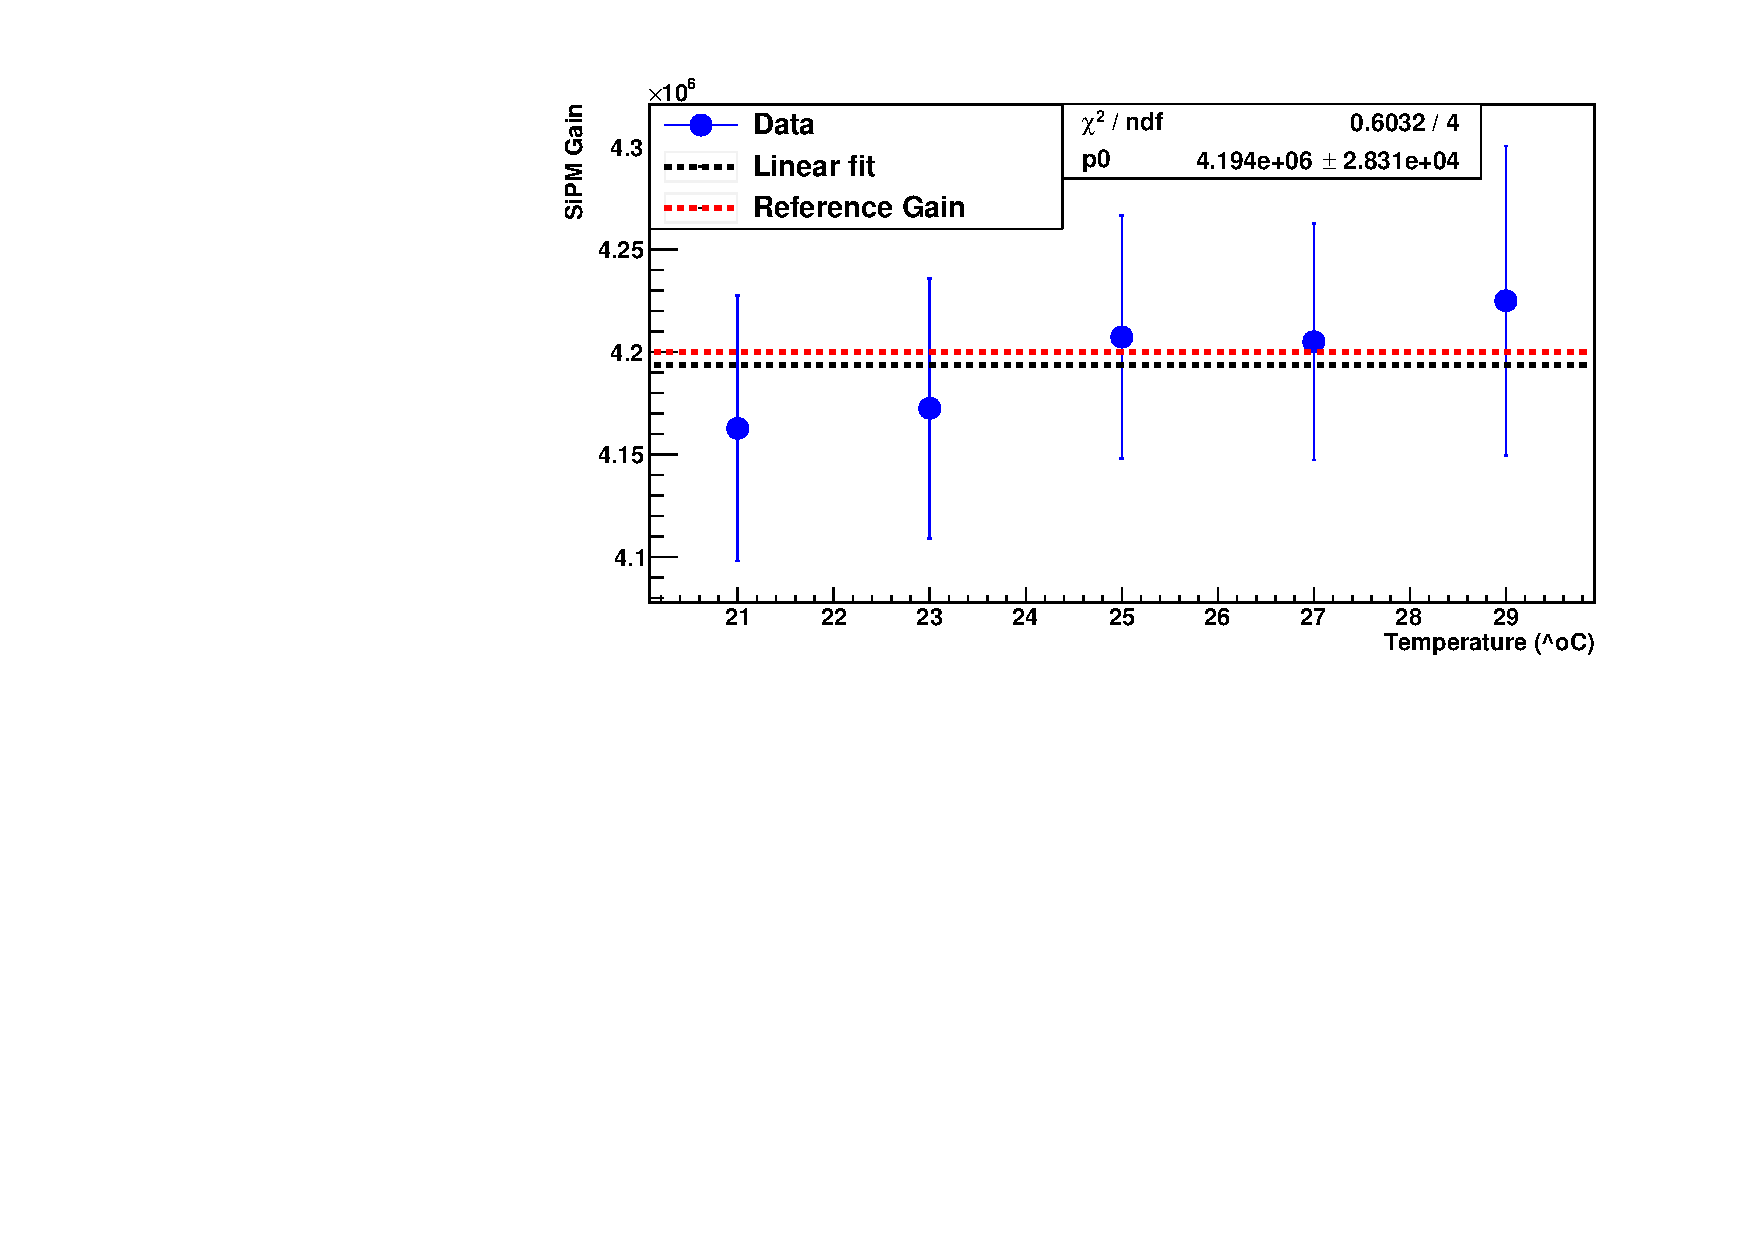
\includegraphics[scale=0.6]{4ResearchAndDevelopments/42SiPM/SiPMGain_Stabilization.pdf}
\caption{SiPM gain as a function of the temperature. The Stabilization method is applied in this experience. \label{fig:SiPMGainStabilization}}
\end{figure}

A red dotted line is included, indicating the value of the SiPM gain to be kept. As it has been proven, the SiPM gain is maintained correctly, which shows that the method of stabilizing the SiPM gain works properly.